\documentclass[tikz,border=6pt]{standalone}
\usepackage{times}
\usepackage{amsmath}
\usetikzlibrary{positioning,arrows.meta,shapes.geometric,fit,matrix,calc}

\definecolor{accent}{RGB}{74,144,217}
\definecolor{accentlight}{RGB}{232,242,251}
\definecolor{rowgray}{RGB}{240,240,240}
\definecolor{linegray}{RGB}{150,150,150}
\definecolor{textgray}{RGB}{55,55,55}
\definecolor{bubblegray}{RGB}{246,246,246}

\tikzset{
  >={Latex[length=2.2mm,width=1.5mm]},
  panel/.style={
    draw=linegray, rounded corners=2pt, inner sep=5pt,
    fill=none, line width=.45pt
  },
  title/.style={
    font=\small\bfseries, text=textgray, anchor=west
  },
  layer/.style={
    draw=linegray, rounded corners=1.5pt, minimum height=5.7mm,
    minimum width=27mm, inner xsep=2.5mm, inner ysep=1mm,
    font=\scriptsize, text=textgray, anchor=west, line width=.35pt
  },
  layeralt/.style={layer, fill=rowgray},
  layerplain/.style={layer, fill=white},
  head/.style={
    draw=accent, fill=accentlight, rounded corners=1.5pt,
    minimum width=7mm, minimum height=5.7mm, inner sep=0pt,
    font=\scriptsize, text=accent, line width=.55pt
  },
  callout/.style={
    draw=linegray, fill=bubblegray, rounded corners=2pt,
    text width=38mm, align=left, inner xsep=3mm, inner ysep=2mm,
    font=\scriptsize, text=textgray, line width=.4pt
  },
  transfer/.style={
    -{Latex[length=2.2mm]}, draw=linegray, line width=.65pt
  },
  result/.style={
    draw=linegray, fill=bubblegray, rounded corners=3pt,
    text width=47mm, align=left, inner xsep=3mm, inner ysep=2.2mm,
    font=\scriptsize, text=textgray, line width=.45pt
  },
  final/.style={
    draw=accent, fill=accentlight, rounded corners=3pt,
    text width=47mm, align=center, inner xsep=3mm, inner ysep=2mm,
    font=\scriptsize, text=textgray, line width=.55pt
  }
}

\begin{document}
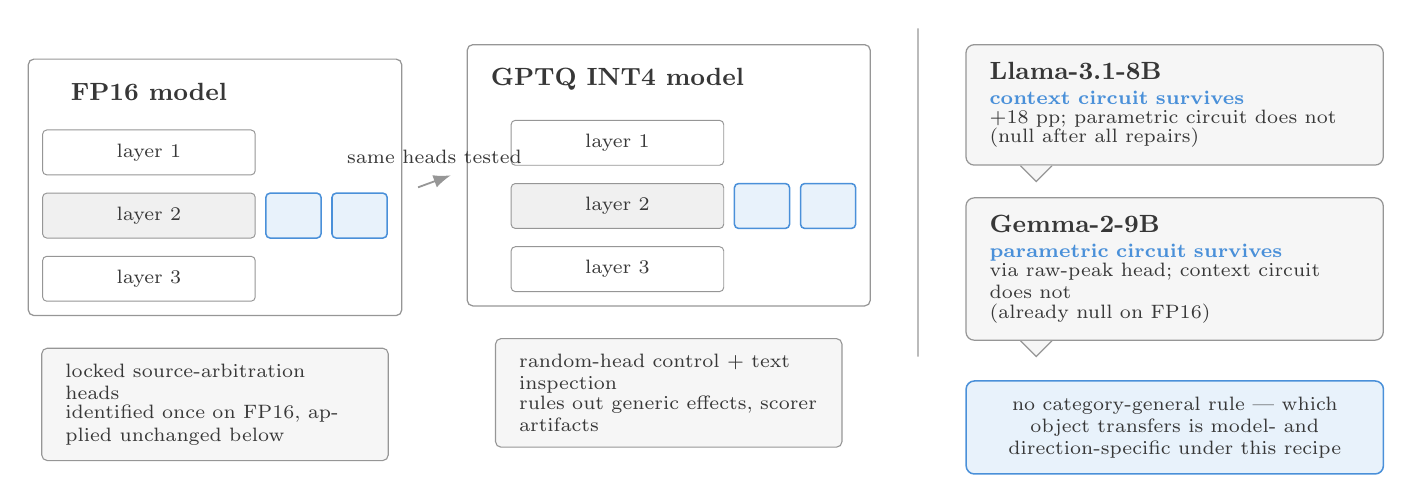
\begin{tikzpicture}[node distance=2.2mm and 7mm]

% FP16 model: the second layer contains the identified heads.
\node[title] (fp-title) {FP16 model};
\node[layerplain, below=2.5mm of fp-title] (fp-l1) {layer 1};
\node[layeralt, below=of fp-l1] (fp-l2) {layer 2};
\node[layerplain, below=of fp-l2] (fp-l3) {layer 3};
\node[head, right=1.2mm of fp-l2.east] (fp-h1) {};
\node[head, right=1.2mm of fp-h1.east] (fp-h2) {};
\node[panel, fit=(fp-title) (fp-l1) (fp-l3) (fp-h2)] (fp-panel) {};
\node[callout, below=4mm of fp-panel] (fp-note)
  {locked source-arbitration heads\\[-1pt]
   \scriptsize identified once on FP16, applied unchanged below};

% GPTQ INT4 model: the same highlighted head locations are tested.
\node[title, right=10mm of fp-panel.north east, anchor=north west] (int-title) {GPTQ INT4 model};
\node[layerplain, below=2.5mm of int-title] (int-l1) {layer 1};
\node[layeralt, below=of int-l1] (int-l2) {layer 2};
\node[layerplain, below=of int-l2] (int-l3) {layer 3};
\node[head, right=1.2mm of int-l2.east] (int-h1) {};
\node[head, right=1.2mm of int-h1.east] (int-h2) {};
\node[panel, fit=(int-title) (int-l1) (int-l3) (int-h2)] (int-panel) {};
\node[callout, below=4mm of int-panel] (int-note)
  {random-head control + text inspection\\[-1pt]
   \scriptsize rules out generic effects, scorer artifacts};

% Transfer arrow.
\draw[transfer] ([xshift=2mm]fp-panel.east) --
  node[above=1mm, font=\scriptsize, text=textgray] {same heads tested}
  ([xshift=-2mm]int-panel.west);

% Right-side outcome panels.
\node[result, right=12mm of int-panel.north east, anchor=north west] (llama)
  {\textbf{\small Llama-3.1-8B}\\[1pt]
   \textcolor{accent}{\textbf{context circuit survives}}\\[-1pt]
   +18 pp; parametric circuit does not\\[-1pt]
   (null after all repairs)};
\node[result, below=4mm of llama] (gemma)
  {\textbf{\small Gemma-2-9B}\\[1pt]
   \textcolor{accent}{\textbf{parametric circuit survives}}\\[-1pt]
   via raw-peak head; context circuit does not\\[-1pt]
   (already null on FP16)};

% Minimal bubble tails and divider.
\draw[linegray, fill=bubblegray, line width=.45pt]
  ($(llama.south west)+(7mm,0)$) -- ++(2mm,-2mm) -- ++(2mm,2mm);
\draw[linegray, fill=bubblegray, line width=.45pt]
  ($(gemma.south west)+(7mm,0)$) -- ++(2mm,-2mm) -- ++(2mm,2mm);
\draw[linegray, line width=.45pt]
  ($(int-panel.north east)+(6mm,2mm)$) -- ($(gemma.south west)+(-6mm,-2mm)$);

\node[final, below=5mm of gemma.south west, anchor=north west] (conclusion)
  {no category-general rule --- which object transfers is model- and
   direction-specific under this recipe};

\end{tikzpicture}
\end{document}
